\chapter{DRIPPING FAUCET}
\label{chap:dripping_faucet}
\mquote{not selectet yet}{...}
    In the previous chapter, we discussed the possibility of swapping a complex and often computationally demanding model for a simpler alternative that behaves similarly. Because the accretion disk is an incredibly complex system, we must also follow this approach and find a suitable and computationally manageable simplification. We chose to employ a relatively simple model of a dripping faucet, which is a reasonably well-understood system known to exhibit non-linear behavior under certain conditions. There are two types of dripping faucet models. 

    For a better understanding of drop formation processes and a more detailed study of fluid behavior, we can construct a model based on Navier-Stokes equations or Lagrange equations. The key roles in such a model, which is referred to as \emph{Fluid Dynamical Model} (FDM), are played by surface tension, viscosity, and gravity \parencite{faucet1999}.   

    The second type of dripping faucet model is called \emph{Mass-Spring Model}, and as its name suggests, it is based on the approximation of the forming drop as a mass hanging on a spring \citep{shaw1984}. It evolves through time, with the steady fluid influx, until it reaches a predefined critical mass. At that moment, part of the drop is separated, the system resets its parameters, and the cycle repeats. 

    Both types are highly sensitive to the amount of fluid that steadily flows in. This parameter is the determining factor of the non-linear behavior of these systems. Depending on the concrete value of inflow, the dripping intervals can be either periodic or get through period-doubling stages to complete aperiodicity. 

\section{Drop equilibrum states}
    \label{sec:drop_equilibrium_states}
    As a prerequisite for dynamical fluid simulations, we need to know the static equilibrium states of hanging drops on a faucet and evaluate the stability of different shapes and sizes. 

    Let us assume a statically hanging axisymmetrical drop with homogenous fluid density $\rho$. According to \citep{faucet1999}, the drop in equilibrium is defined as follows. The pressure inside the drop is 
    
    % 4.2
    \begin{equation}
        P = \rho g z,
    \end{equation}

    where $z$ represents the vertical coordinate, and $g$ is gravitaional acceleration. The following expression describes the pressure difference between the inside and outside of the drop

    % 4.3
    \begin{equation}
        P = \Gamma \left( \frac{1}{R_1} + \frac{1}{R_2}  \right),
    \end{equation}

    where the surface tension is represented by $\Gamma$. $R_1$ and $R_2$ are the curvature radii of the drop's surface that, for the axisymmetric drop, are

    % 4.5
    \begin{align}
    \begin{split}
        \frac{1}{R_1} &= - \frac{\diff \theta}{\diff s}, \\
        \frac{1}{R_2} &= \frac{\cos \theta}{r}.
    \end{split}    
    \end{align}

    Figure \ref{fig:drop_equilibrum_definition} explains in detail the variables used to calculate the shape of the hanging drop.
    
    \begin{figure}[H]
    \begin{center}
        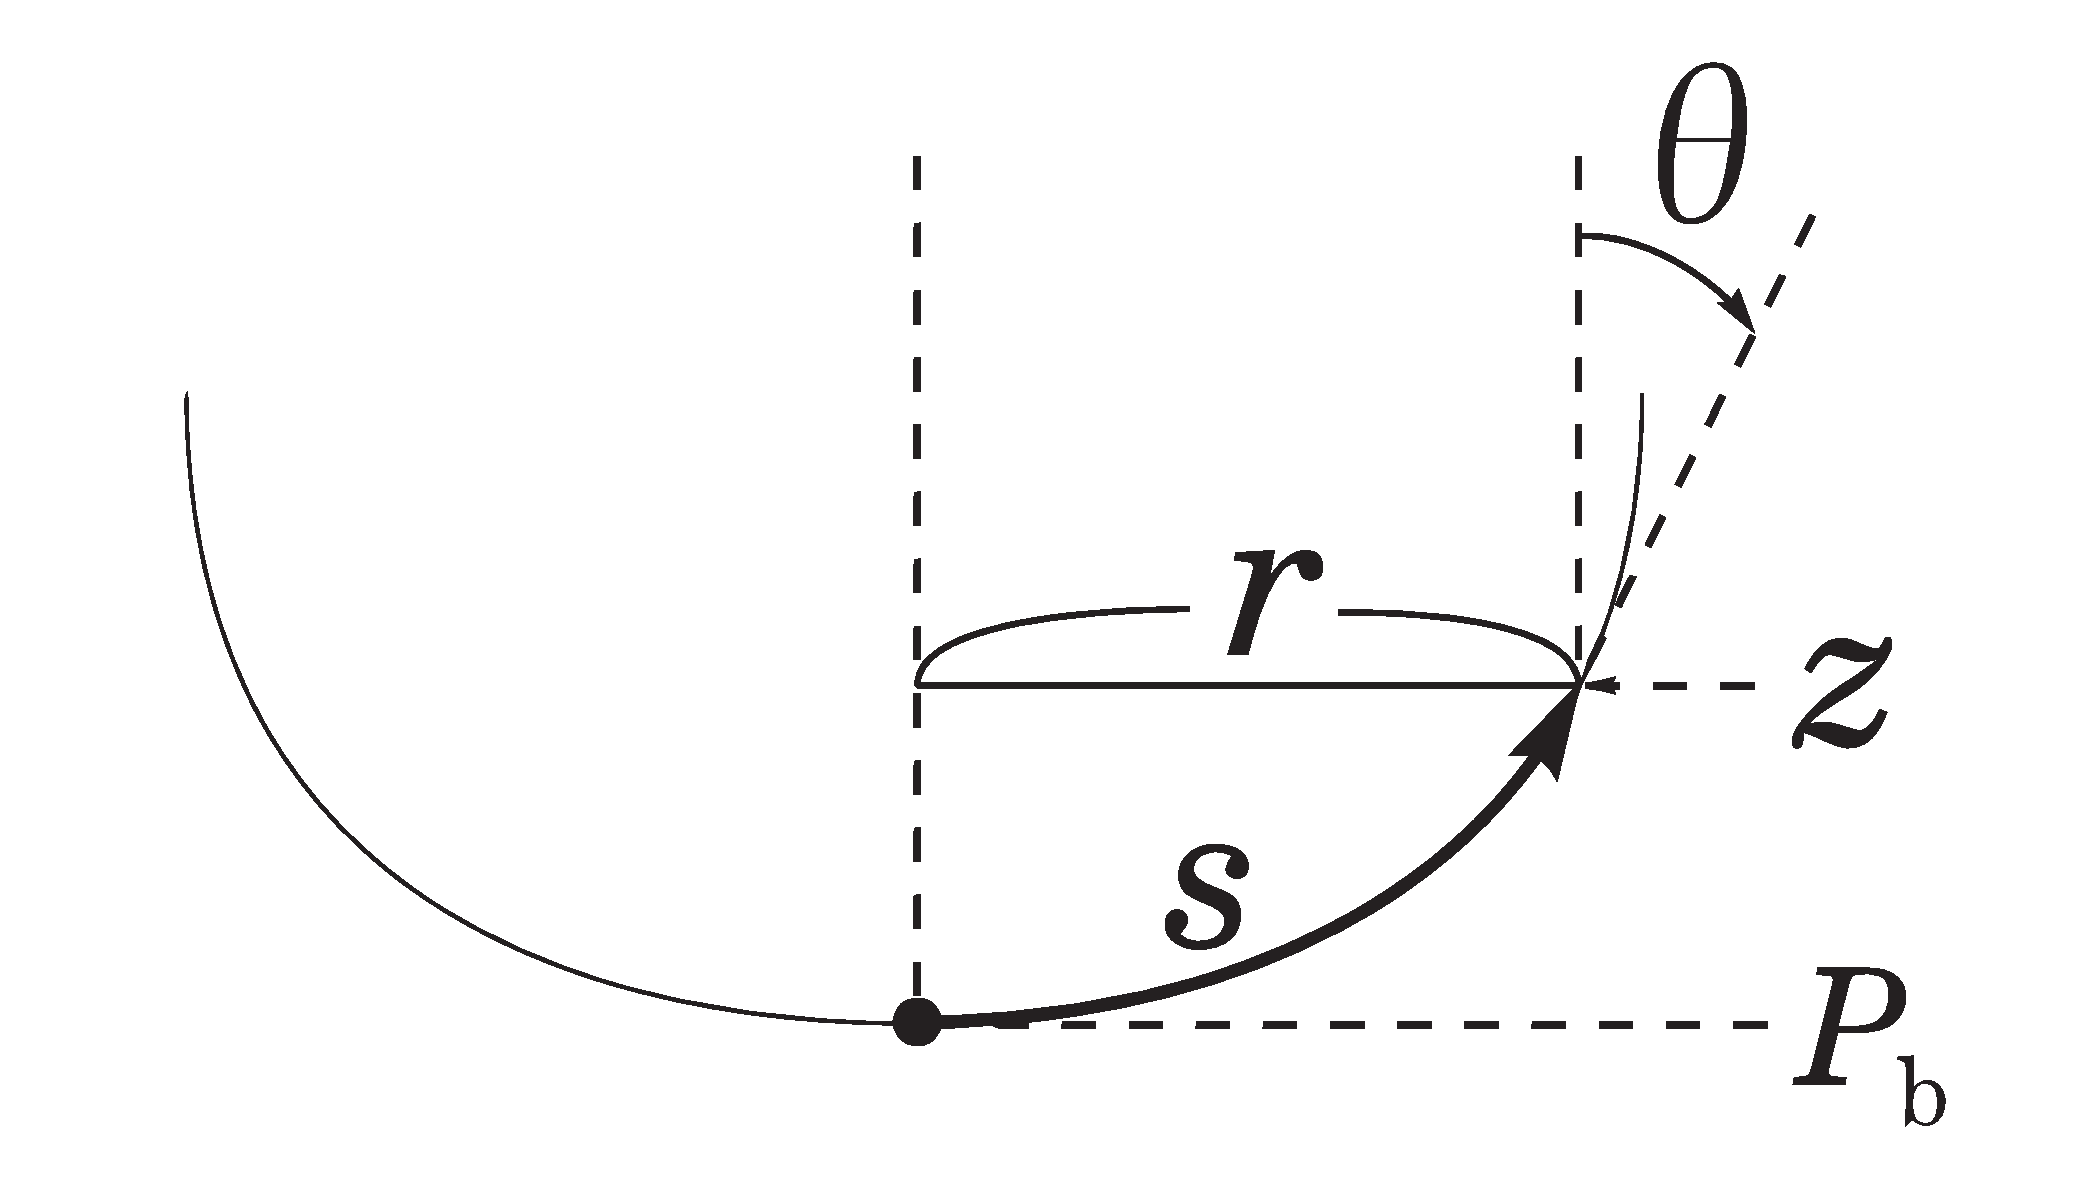
\includegraphics[width=0.75\columnwidth]{img/drop_equilibrum_definition.pdf}
    \end{center}
    \caption{Definition of variables for the hanging drop system. Taken from \citep{faucet1999}} 
    \label{fig:drop_equilibrum_definition}
    \end{figure}

    % 4.4
    \begin{align}
    \begin{split}
        m_0 &= \rho l_0^3 = 0.02 \si{\gram}, \\
        P_0 &= \sqrt{\rho g \Gamma} = 270 \si{dyne \cdot \cm^{-2}}, \\
        l_0 &= \sqrt{\frac{\Gamma}{\rho g}} = 0.27 \si{\cm}, \\
        t_0 &= 0.017 \si{\second}.
    \end{split}
    \label{eq:base_units_drop}
    \end{align}

    Defined by equations \eqref{eq:base_units_drop} are the base units of mass, pressure, and length, that sets $\Gamma = \rho = g = 1$; assuming the medium is water at $20 \si{\celsius}$. The drop's shape is then described by a set of ODE's \eqref{eq:drop_equilibrum_odes}, that are solved numerically, with the use of the initial conditions: $z(0) = P_{\mathrm{b}}$, $\theta(0) = \pi / 2$, and $r(0) = 1 \cdot 10^{-20}$

    % 4.6
    \begin{align}
    \begin{split}
        \frac{\diff r}{\diff s} &= \sin \theta, \\
        \frac{\diff z}{\diff s} &= - \cos \theta, \\
        \frac{\diff \theta}{\diff s} &= \frac{\cos \theta}{r} - z.
    \end{split}
    \label{eq:drop_equilibrum_odes}
    \end{align}

    Figure \ref{fig:plot_drop_equilibrium_ceiling} shows multiple equilibrium state solutions for different values of pressure $P_{\mathrm{b}}$ at the bottom of the drop.

    \begin{figure}[H]
    \begin{center}
        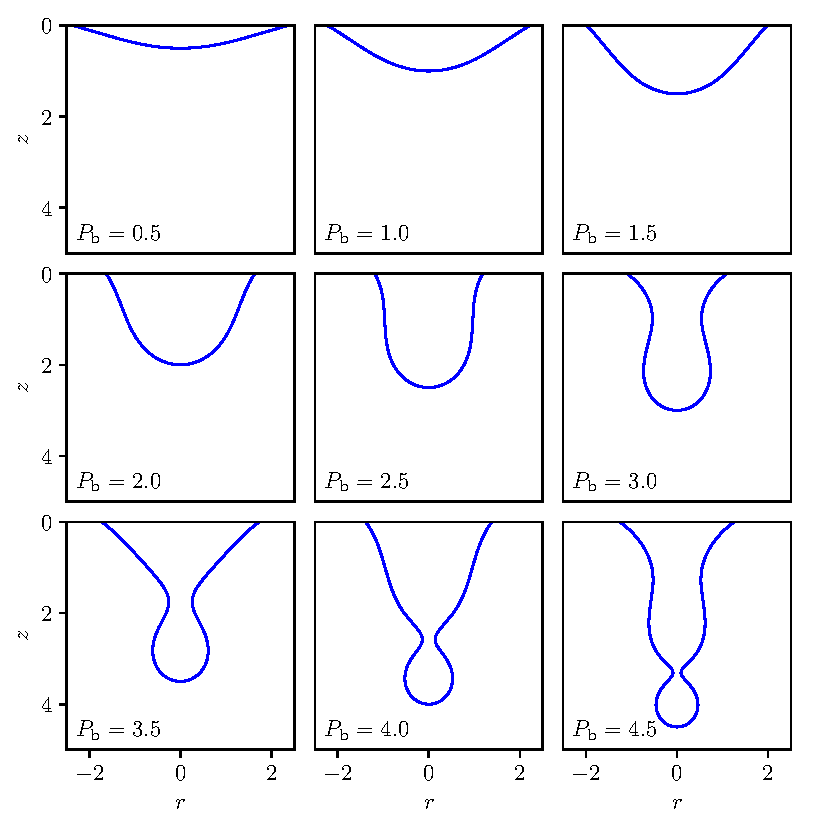
\includegraphics[width=1.0\columnwidth]{img/plot_drop_equilibrium_ceiling.pdf}
    \end{center}
        \caption{Examples of unbounded static equilibrium drop states, which are solutions of ODE's \eqref{eq:drop_equilibrum_odes} for different values of pressure $P_{\mathrm{b}}$ on the bottom of the drop.}
    \label{fig:plot_drop_equilibrium_ceiling}
    \end{figure}
    
    Similarly to solutions shown in Figure \ref{fig:plot_drop_equilibrium_ceiling}, we can bound the equilibrium states to a faucet of chosen radius $r_{\mathrm{a}}$. This is done by using the same solutions, finding a point of the closest match with the chosen boundary (i.e., the faucet), and shifting $z$ coordinates accordingly. Figure \ref{fig:plot_drop_equilibrium_faucet} shows drop solutions bounded to a faucet. Both unbounded and bounded examples are done for the same initial conditions. 

    \begin{figure}[H]
    \begin{center}
        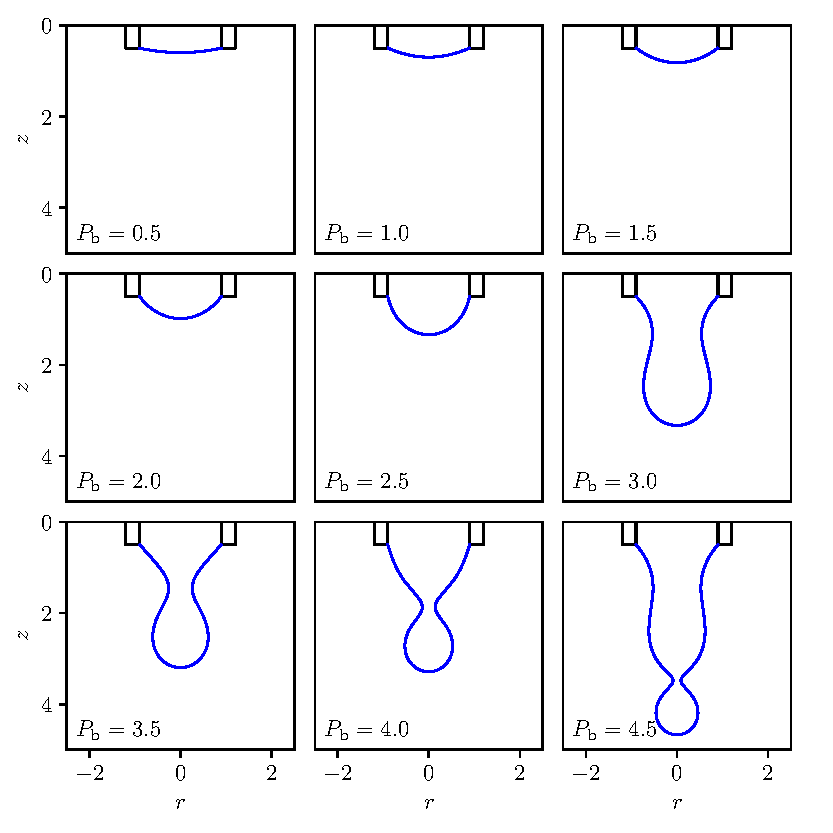
\includegraphics[width=1.0\columnwidth]{img/plot_drop_equilibrium_faucet.pdf}
    \end{center}
        \caption{Examples of static equilibrium drop states bounded to a faucet, which is solutions of ODE's \eqref{eq:drop_equilibrum_odes} for different values of pressure $P_{\mathrm{b}}$ on the bottom of the drop.}
    \label{fig:plot_drop_equilibrium_faucet}
    \end{figure}

    We assume, as is also self-evident from Figures \ref{fig:plot_drop_equilibrium_ceiling} and \ref{fig:plot_drop_equilibrium_faucet}, that not all of these solutions are stable and therefore usable as initial states of FDM. \emph{Stable}, in this sense, means that the drop shape (i.e., particular solution) stays statically hanging on the faucet, assuming there is no fluid inflow. We can distinguish the stable and unstable solutions based on the relation between drop' volume $V_{\mathrm{d}}$ and the pressure $P_{\mathrm{b}}$ 

    \begin{equation}
        V_{\mathrm{d}} = f(P_{\mathrm{b}}) 
    \end{equation}

    \begin{figure}[H]
    \begin{center}
        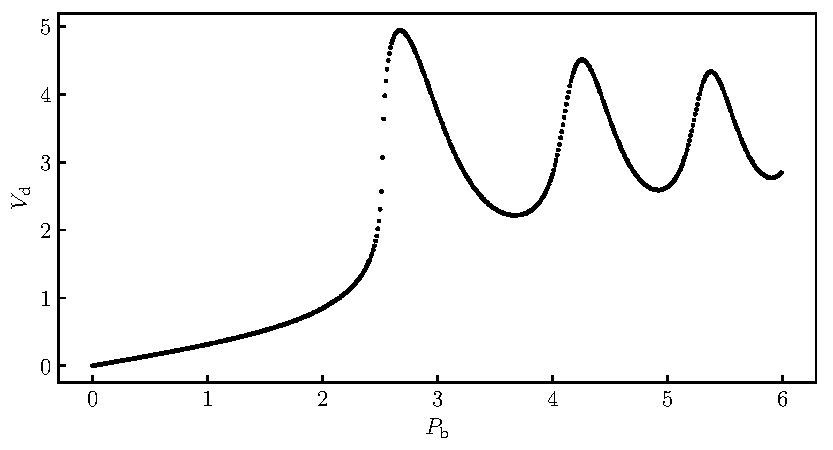
\includegraphics[width=1.0\columnwidth]{img/plot_drop_equilibrium_faucet_pv.pdf}
    \end{center}
        \caption{Static equilibrium solutions of drop shapes hanging on a faucet or radius $r_{\mathrm{a}} = 0.952$. Every point of the solutions curve represents one solution in the interval $P_{\mathrm{b}} \in \langle 1 \cdot 10^{-20}, 6.0 \rangle$.} 
    \label{fig:plot_drop_equilibrium_faucet_pv}
    \end{figure}
        

    As shown by \citep{padday1973}, there is only one stable solution for a given value of the drop's volume. Figure \ref{fig:plot_drop_equilibrium_faucet_pv} demonstrates that for different initial values of $P_{\mathrm{b}} \in \langle 1 \cdot 10^{-20}, 6.0 \rangle$, there are multiple solutions of the same drop's volume. Only the solutions in the interval

    \begin{equation}
        P_{\mathrm{b}} \in \langle 1 \cdot 10^{-20}, 2.67 \rangle,
    \end{equation}

    are the stable ones. Solutions shown in Figure \ref{fig:plot_drop_equilibrium_faucet_pv} are all done assuming the boundary to a faucet with radius $r_{\mathrm{a}}$. This interval of stable drop shapes also provides us with the maximum stable volume of the hanging drop for a particular faucet radius. In the case of $r_{\mathrm{a}} = 0.952$ the maximum stable volume is $V_{\mathrm{d}} = 4.95$.

\section{Fluid dynamical model (FDM)}
    The theory behind drop formation and breakup is a surprisingly recent invention, even though it concerns an everyday phenomenon. However, J. Eggers' scaling theory is universally applicable for viscous axisymmetrical drop formation \citep{eggers1993}, which was later used as a basis for dynamical drop simulations done by \citep{faucet1999}. In the following sections, we will go over the process of modeling the process of FDM. Although this more complex dripping faucet model is more suitable for studying short-term behavior and detailed shapes of forming drops, it is also a precursor for a better understanding the spring-like MSM models discussed later in this chapter.

\subsection{Diskretized FDM Lagrangian}
    The starting point of the simulation is the drop shape in the state of equilibrium (see Section \ref{sec:drop_equilibrium_states}); in particular, the equilibrium solution with the highest stable drop volume $V_{\mathrm{d}}$ for the chosen faucet radius $r_{\mathrm{a}}$. The reason is that as we add more fluid to the system, its path to reaching the critical mass, and therefore the drop breakup, will be the shortest.

    Let us start by defining the Lagrangian for the drop system
    
    % 4.9
    \begin{equation}
        \mathcal{L} = E_{\mathrm{k}} - U_{\mathrm{g}} - U_{\Gamma},
    \end{equation}

    where $E_{\mathrm{k}}$ represents the total kinetic energy of the drop, $U_{\mathrm{g}}$ its total potential energy and $U_{\Gamma}$ its total surface energy. Discretization of the system is done by splitting the drop into $M$ number of disks with equal length along drops surface $\Delta s$ (see. Figure \ref{fig:drop_equilibrum_definition}). The disk has a mass

    \begin{equation}
        m_j = \rho \Delta \xi_j,
    \end{equation}

    where $\Delta \xi_j$ is the volume of particular disk. Because the fluid density is defined as $\rho = 1$, the mass of a single disk is simply

    \begin{equation}
        m_j \equiv \Delta \xi_j.
    \end{equation}

    Therefore the total kinetic energy of the drop system expressed as a sum of individual disks is 

    %4.10
    \begin{equation}
        E_{\mathrm{k}} = \frac{1}{2} \sum^M_{j=1} \Delta \xi_j \dot{z}_j^2.
    \end{equation}

    Similarly, the potential energy is a sum of its values for all disks

    %4.11
    \begin{equation}
        U_{\mathrm{g}} = -g \sum^M_{j=1} \Delta \xi_j z_j,
    \end{equation}

    where $g$ is the gravitational acceleration. The expression for surface energy is approximated by 

    %4.12
    \begin{equation}
        U_{\Gamma} = \Gamma S,
    \end{equation}

    where $S$ represents the total surface area of the drop. The computation of the surface energy comes down to determining the surface area $S$ as a sum of individual disk surfaces. We can approximate the surface area $S_j$ of a single disk as the surface area of the truncated cone's outer shell in the interval $\langle (z_{j+1} + z_j) / 2; (z_j + z_{j-1}) / 2 \rangle$, which then is

    %4.13
    \begin{equation}
        S_j = \pi (r_j + r_{j+1}) \sqrt{\frac{1}{4} (z_{j+1} - z_{j-1})^2 + (r_j - r_{j+1})^2}.
    \end{equation}

    Assuming the average radii of disks
    
    %4.18
    \begin{equation}
        r_j = \sqrt{\frac{\Delta \xi_j}{\pi (z_j - z_{j-1})}}.
    \end{equation}

    Therefore the surface energy is then expressed as

    \begin{equation}
        U_{\Gamma} = \Gamma \sum_{j=1}^M S_j(z_{j-1}, z_j, z_{j+1}),
    \end{equation}

    which gives us the final Lagrangian of the discretized drop system

    \begin{equation}
        \mathcal{L} = E_{\mathrm{k}}(\dot{z}_1, ..., \dot{z}_M) - U_{\mathrm{g}}(z_1, ..., z_M) - U_{\Gamma}(z_1, ..., z_M)
    \end{equation}

\subsection{FDM simulation}
    To conduct the simulation, the equations of motion for the drop system are calculated from

    \begin{equation}
        \frac{\diff}{\diff t} \frac{\partial \mathcal{L}}{\partial \dot{z}_j} = \frac{\partial \mathcal{L}}{\partial z_j} + \frac{1}{2} \frac{\partial \dot{E}_{\mathrm{k}}}{\partial \dot{z}_j}
    \end{equation}

    where $\mathcal{L}$ is the previously obtained Langrangian of the drop as a sum of its disk discretization in the interval $j \in \langle 1; M \rangle$. Examples of the simulation results done by \citep{faucet1999} are shown in Figure \ref{fig:plot_fdm_simulation}.
    
    \begin{figure}[H]
    \begin{center}
        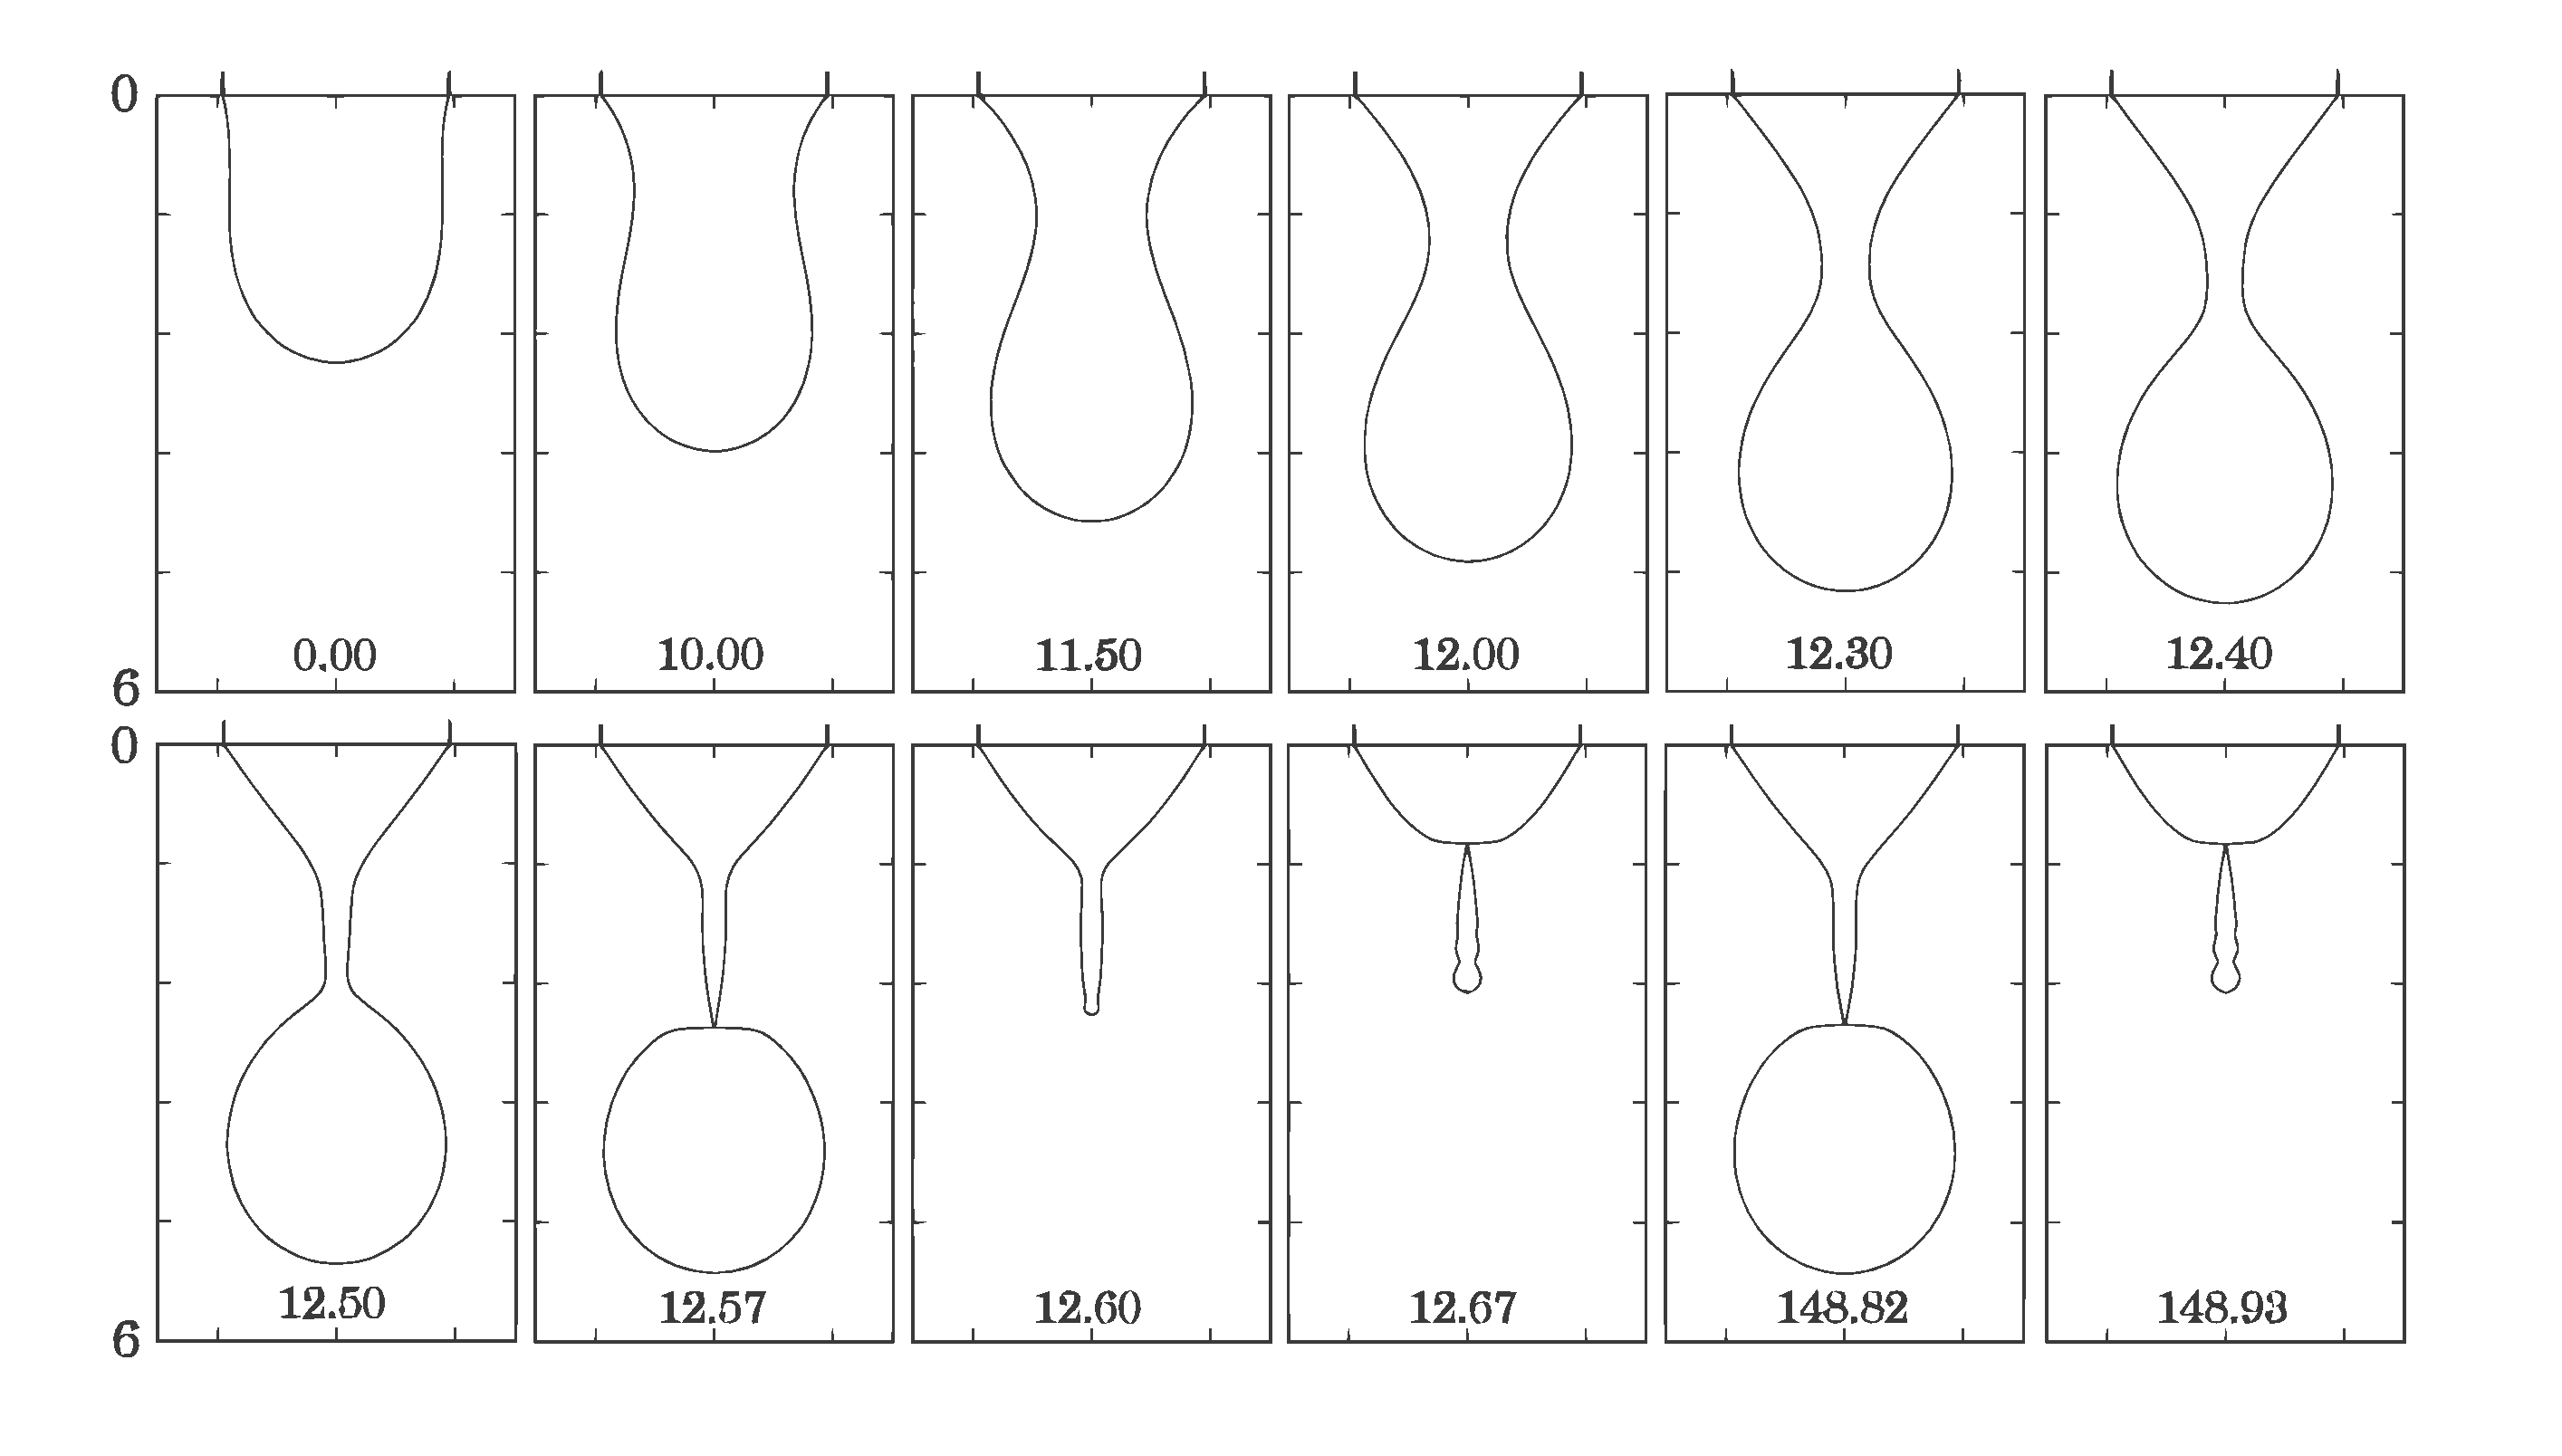
\includegraphics[width=1.0\columnwidth]{img/plot_fdm_simulation.pdf}
    \end{center}
        \caption{Time development of drop shape for the faucet radius $r_{\mathrm{a}} = 0.952$. Taken from \citep{faucet1999}.}
    \label{fig:plot_fdm_simulation}
    \end{figure}

\section{Mass-spring model (MSM)} \label{section:msm}
    \begin{align}
    \begin{split}
        \D{}{t} \left(m \D{z}{t}\right) &= -kz - \gamma\D{z}{t} + mg, \\
        \D{m}{t} &= Q,
    \end{split}
    \label{eq:msm_original_odes}
    \end{align}
    %
    % where $z$ represents the position of the hanging mass $m$. $Q$ is \emph{mass influx}, and it is the main determining parameter of MSM because by choosing a specific value of $Q$, we can drastically alter our model's behavior, as shown in \citep{msmm1999}. Parameter $\gamma=0.05$ is the dampening ratio, and $k$ is the stiffness of the imaginary spring defined as
    %
    \begin{equation}
        \begin{aligned}
            & k~=
            \begin{cases}
                -11.4\ m + 52.5 \hspace{10mm} (m < 4.61) \\
                \hspace{12mm} 0 \hspace{20mm} (m \ge 4.61 ).
            \end{cases}
        \end{aligned}
        \label{eq:spring_stiffness}
    \end{equation}
    %
    % Relations expressed by \eqref{eq:spring_stiffness} and the value of $\gamma$ were obtained experimentally by \citep{shaw1984} and provide a good description for the real-world behavior of drops and leaky faucet. Simply put, \eqref{eq:spring_stiffness} means that if the mass contained in the MSM exceeds the value of $m = 4.61$, the matter essentially goes into free fall.

    \begin{equation}
        z_c = 5.5.
        \label{eq:z_critical_model}
    \end{equation}

\section{Dripping handrail models}


